\setcounter{chapter}{-1}
\chapter{Preface}
\section{What is integrability?}
There is no universal definition and depends on context and model. However, the harmonic oscillator, which can be approximation of some complete model, is integrable.

\section{FPUT paradox}
In year 1954, Los Almos, USA, there was a brand new computer MANIAC I. Fermi had published an article in 1923 "Beweis dass mechanisches Normalsystem im Allgemein quasiergodisch ist". Here ergodic means equipartion of energy among different degrees of freedom. With this new machine, he did numerical experiment on how long it takes until equipartition is reached. A simple model would be a discrete vibrating string. The Hamiltonian is 
\begin{equation*}
	H(p, q) =\frac{1}{2} \sum_{i=1}^{L}  p_i^2 + \frac{1}{2} \sum_{i=1}^{L} (q_i - q_{i-1})^2 - 2\alpha \sum_{i=1}^{L} (q_i - q_{i-1})^3
\end{equation*}
with the fixed boundary condition $q_0 = q_L = 0$. By defining the normal mode coordinates
\begin{align*}
	Q_k &= \sqrt{\frac{2}{L+1}} \sum_{i=1}^{L} \sin(\frac{ik\pi}{L+1}) q_i, \\
	P_k &= \sqrt{\frac{2}{L+1}} \sum_{i=1}^{L} \sin(\frac{ik \pi}{L+1}) p_i,
\end{align*}
the Hamiltonian becomes
\begin{equation}
	H(P, Q) = \frac{1}{2} \sum \left( P_k^2 + \omega_k^2 Q_k^2 \right)  + \alpha V_e(Q),
\end{equation}
with 
\begin{equation*}
\omega_k = 2 \sin(\frac{k\pi}{2(L+1)})	.
\end{equation*}
The first term in the Hamiltonian is a good approximation for energy per site for small $\alpha$ and the last term is the non-linear term. One can define the average energy per site
\begin{equation}
	\bar{E}_k = \frac{1}{t_0} \int_t^{t_0} E_k^0 (t) \dd{t}
\end{equation}
The expectation (from ergodicity or equipartion) is $\lim_{t\rightarrow \infty} \bar{E}_k(t_0) = \epsilon$ for all $k$.

In the FPUT test, some initial energy is given to mode $k=1$ and wait until equilibrium is reached. The results are shown in figure
\begin{figure}[ht]
	\centering
	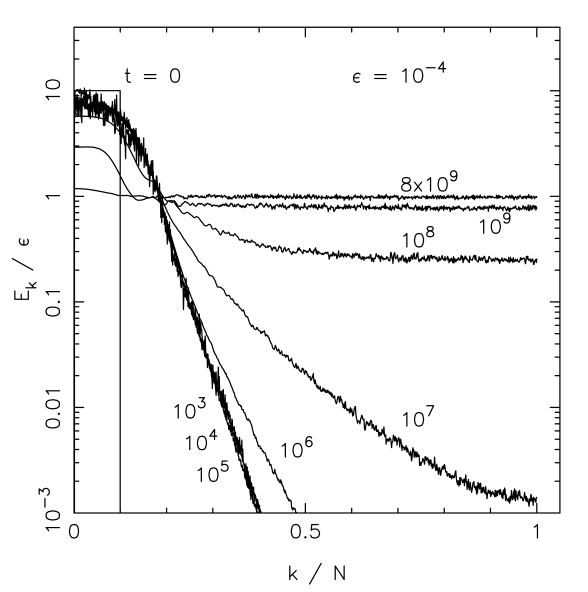
\includegraphics[width=0.4\textwidth]{./figs/FPUT-1.png}%
	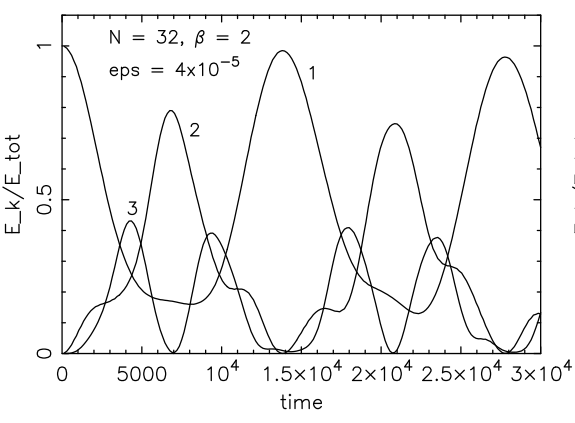
\includegraphics[width=0.5\textwidth]{./figs/FPUT-2.png}
	\caption{Averaged energy spectrum of normal modes $\bar{E}_k (T)$ plotted against $k/N$ at selected times $T$ and instantaneous values $E_k(t)$ for modes $k=1, 2, 3$ \cite{benettinFermiPastaUlamProblemIts2013}.}
	\label{fig:}
\end{figure}

System shows periodicity instead of equipartition of energy! Why? Are there some hidden symmetries? Still today, there is no satisfactory explanation for FPUT paradox. The FPUT system is close to a class of so-called \textit{integrable models}, whose a number of (hidden) symmetries, roughly speaking, is the same as the degrees of freedom. 

One obtains FPUT model by introducing perturbation to harmonic oscillator (which is integrable). By truncating FPUT model, one has Toda chain. Taking the continuum limit, FPUT model leads to Korteweg-de Vries (KdV) equation, which is integrable. This lecture is about these integrable models with ``large'' number of symmetries, about mathematical formulation and implications.

About literacy ``integrable'': There is possibility to integrate equation of motion to obtain a solution in a form as closed as possible (may require some extra steps).
